% !TEX root = ../om_ts_01.tex

\begin{frame} % frame name
	
	\videotitle{Series Characteristics}
	
\end{frame}



\begin{frame}{Series Characteristics: Plan}
	\begin{itemize}[<+->]
		\item Sample autocorrelation
		\item Sample partial autocorrelation
		\item STL features
	\end{itemize}
	
\end{frame}

\begin{frame}{Tasks for multiple series}
	\begin{itemize}
		\item Classify the new series into one of the existing classes
		\item Understand which series are close to each other
		\item Cluster series into an unknown set of clusters
	\end{itemize}
	\pause
	\alert{How to solve?}
	\begin{enumerate}[<+->]
		\item Generate \alert{features} for each series
		\item Apply the algorithms for cross data to the obtained features
	\end{enumerate}
	\pause
	Classify using random forest;
	
	Measure distance using the Mahalanobis metric;
	
	Cluster using hierarchical clustering
	
\end{frame}


\begin{frame}{Creating features}
	
	Two \alert{sets} of features:
	\begin{itemize}[<+->]
		\item Sample ACF (\alert{autocorrelation function}, AutoCorrelation Function)
		\item Sample PACF (\alert{partial} autocorrelation function, Partial ACF)
	\end{itemize}
	
	\pause
	From \alert{one} series we get:
	
	$ACF_1$, $ACF_2$, $ACF_3$, \ldots
	
	$PACF_1$, $PACF_2$, $PACF_3$, \ldots
\end{frame}


\begin{frame}{ACF}
	
	\begin{block}{Sample ACF}
		Let's evaluate a set of paired regressions:
		\[
		\hat y_t = \hat\beta_1 + \hat\beta_2 y_{t-1}, \quad ACF_1 = \hat\beta_2;
		\]
		\pause
		\[
		\hat y_t = \hat\beta_1 + \hat\beta_2 y_{t-2}, \quad ACF_2 = \hat\beta_2;
		\]
		\pause
		\[
		\hat y_t = \hat\beta_1 + \hat\beta_2 y_{t-k}, \quad ACF_k = \hat\beta_2
		\]
	\end{block}
	
	\pause
	\alert{Meaning}
	$ACF_2$: How many units is $y_t$ above average on average if $y_{t-2}$ is one unit above average.
	
\end{frame}


\begin{frame}{Series and its ACF}
	
	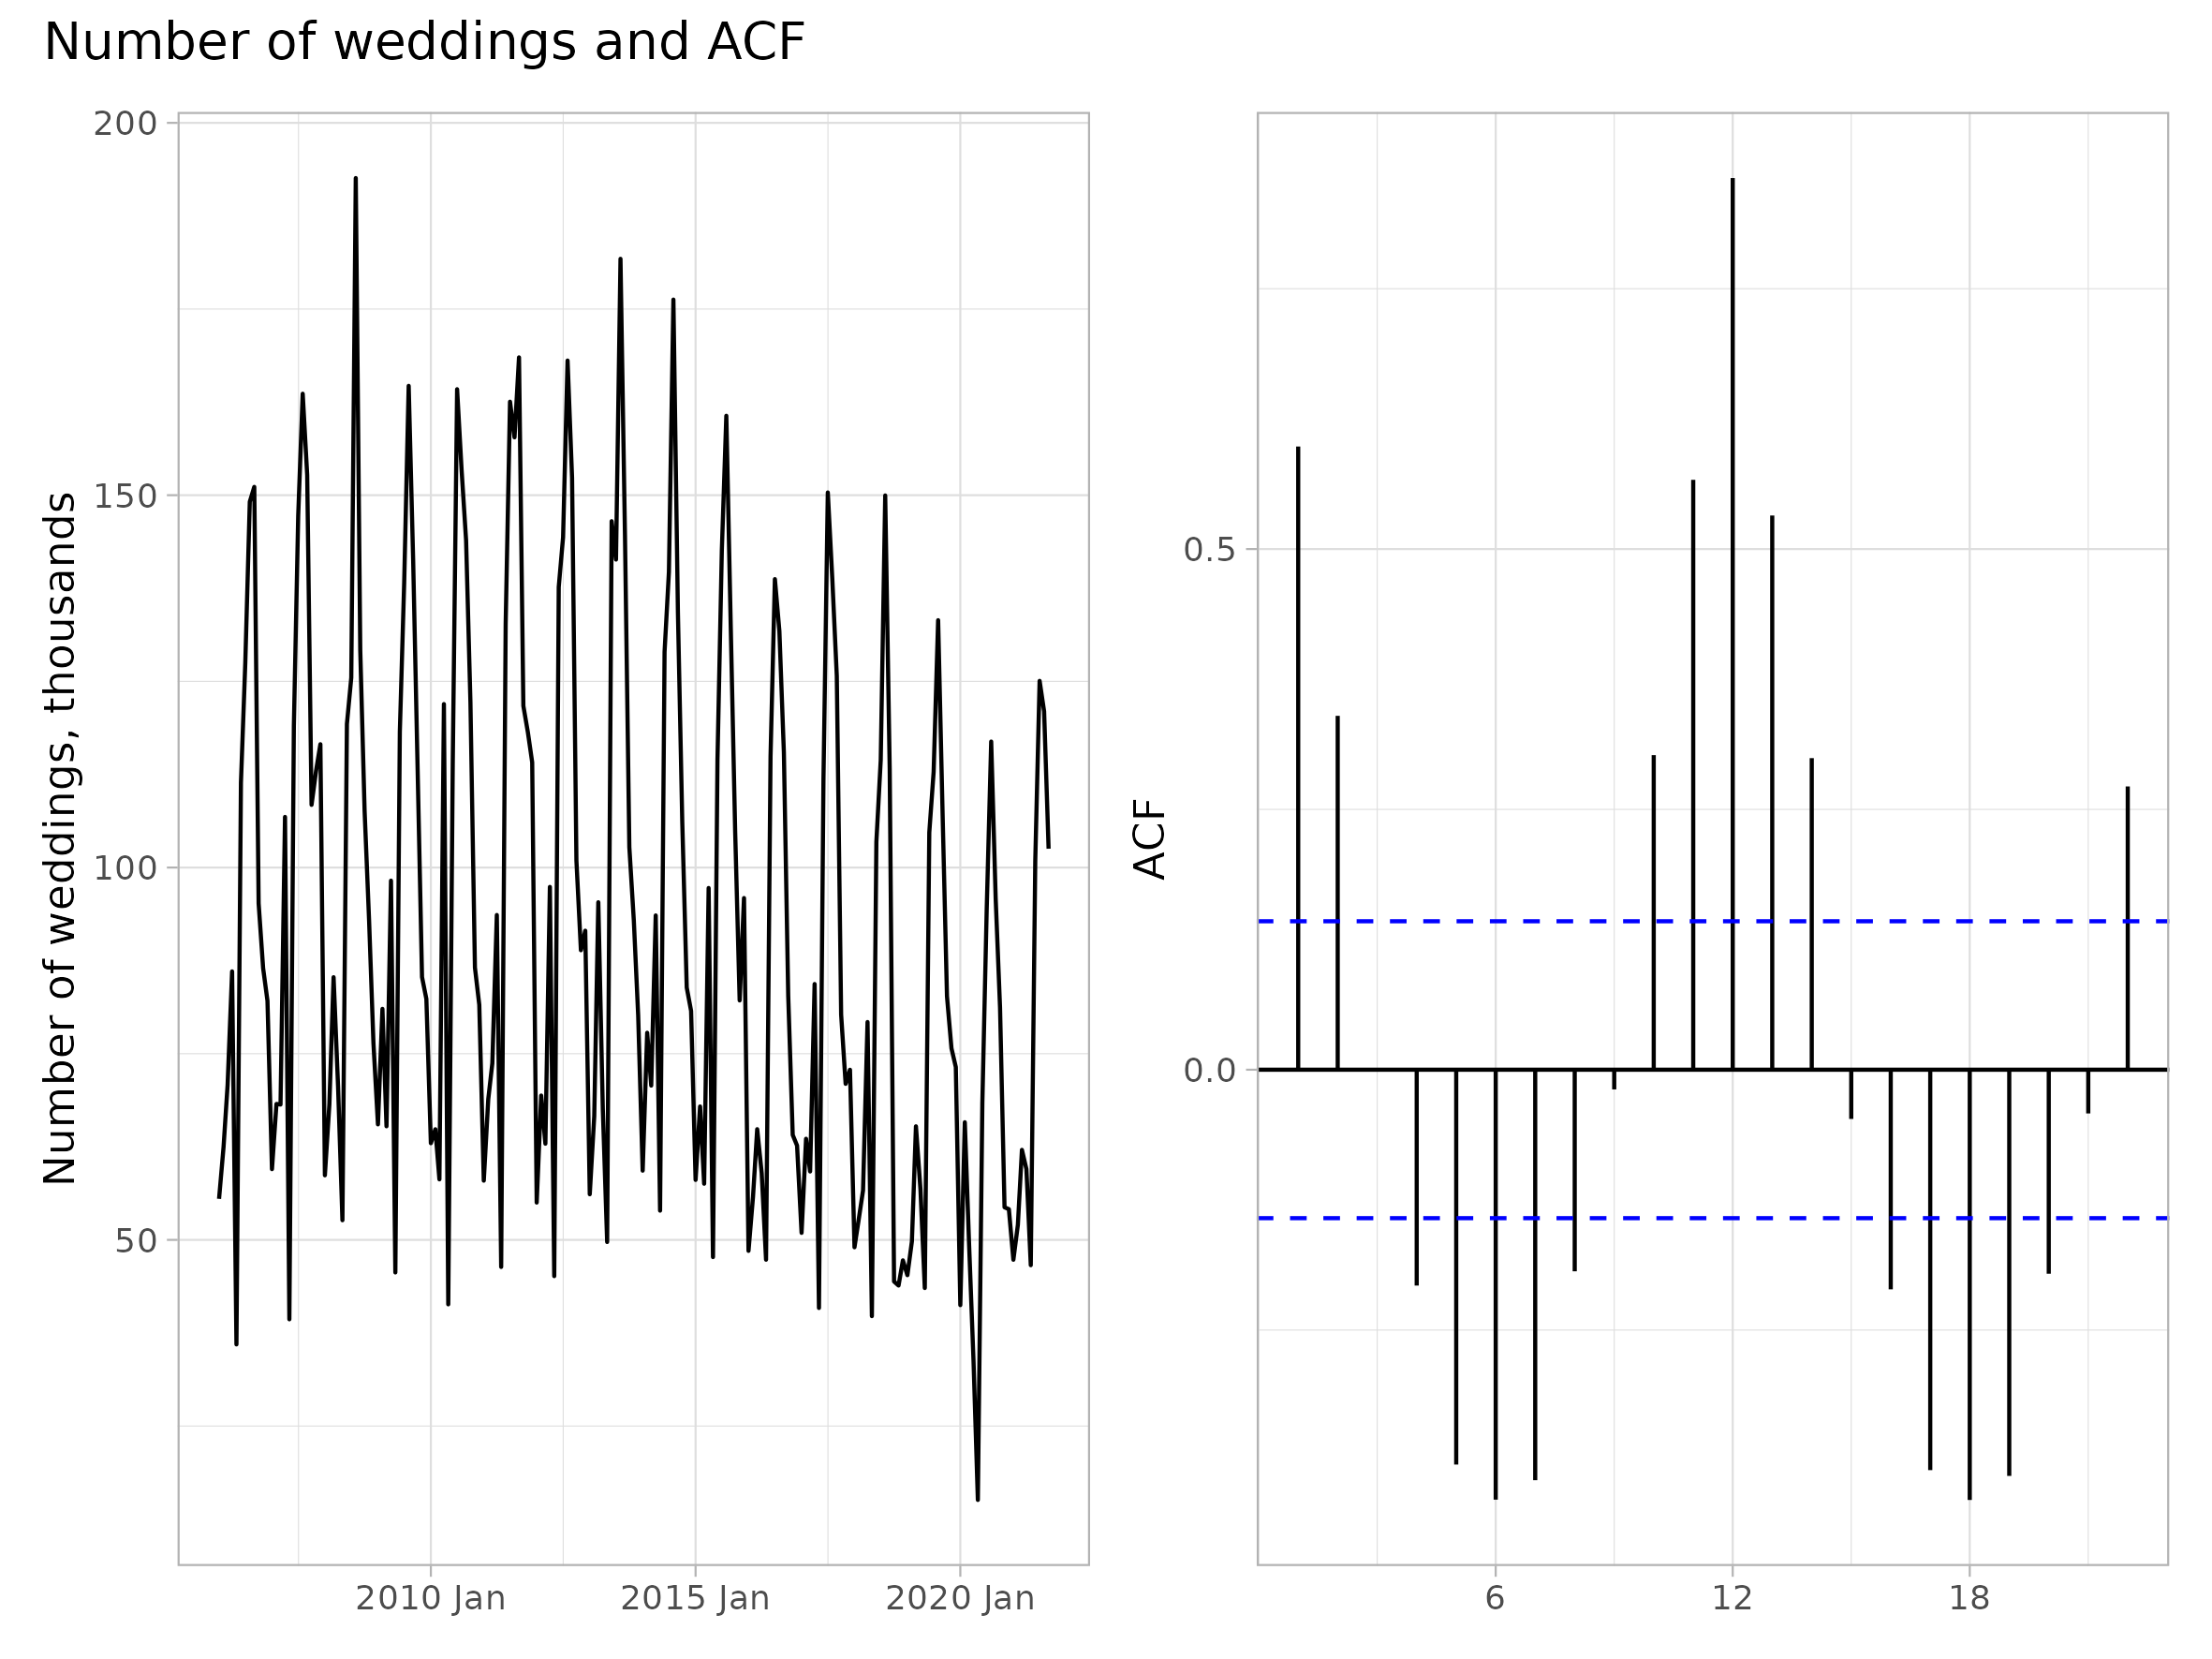
\includegraphics[width=\textwidth]{pictures/om_ts_01-120.png}
	
\end{frame}

\begin{frame}{Why is ACF a correlation?}
	
	\alert{Classic definition}
	
	\begin{block}{Sample ACF}
		$ACF_k$ — sample correlation between series $y_t$ and series $y_{t-k}$
	\end{block}
	
	\pause
	The difference between the definitions is \alert{small}
	
\end{frame}


\begin{frame}{PACF}
	
	\begin{block}{Sample PACF}
		Let's evaluate a set of multiple regressions:
		\[
		\hat y_t = \hat\alpha + \hat\beta_1 y_{t-1}, \quad PACF_1 = \hat\beta_1;
		\]
		\pause
		\[
		\hat y_t = \hat\alpha + \hat\beta_1 y_{t-1} + \hat\beta_2 y_{t-2}, \quad PACF_2 = \hat\beta_2;
		\]
		\pause
		\[
		\hat y_t = \hat\alpha + \hat\beta_1 y_{t-1} + \ldots + \hat\beta_k y_{t-k}, \quad PACF_k = \hat\beta_k
		\]
	\end{block}
	
	\pause
	\alert{Meaning}
	$PACF_2$: how many units is $y_t$ above average on average if $y_{t-2}$ is one unit above average,
	and $y_{t-1}$ is at the middle level
	
\end{frame}

\begin{frame}{Series and its PACF}
	
	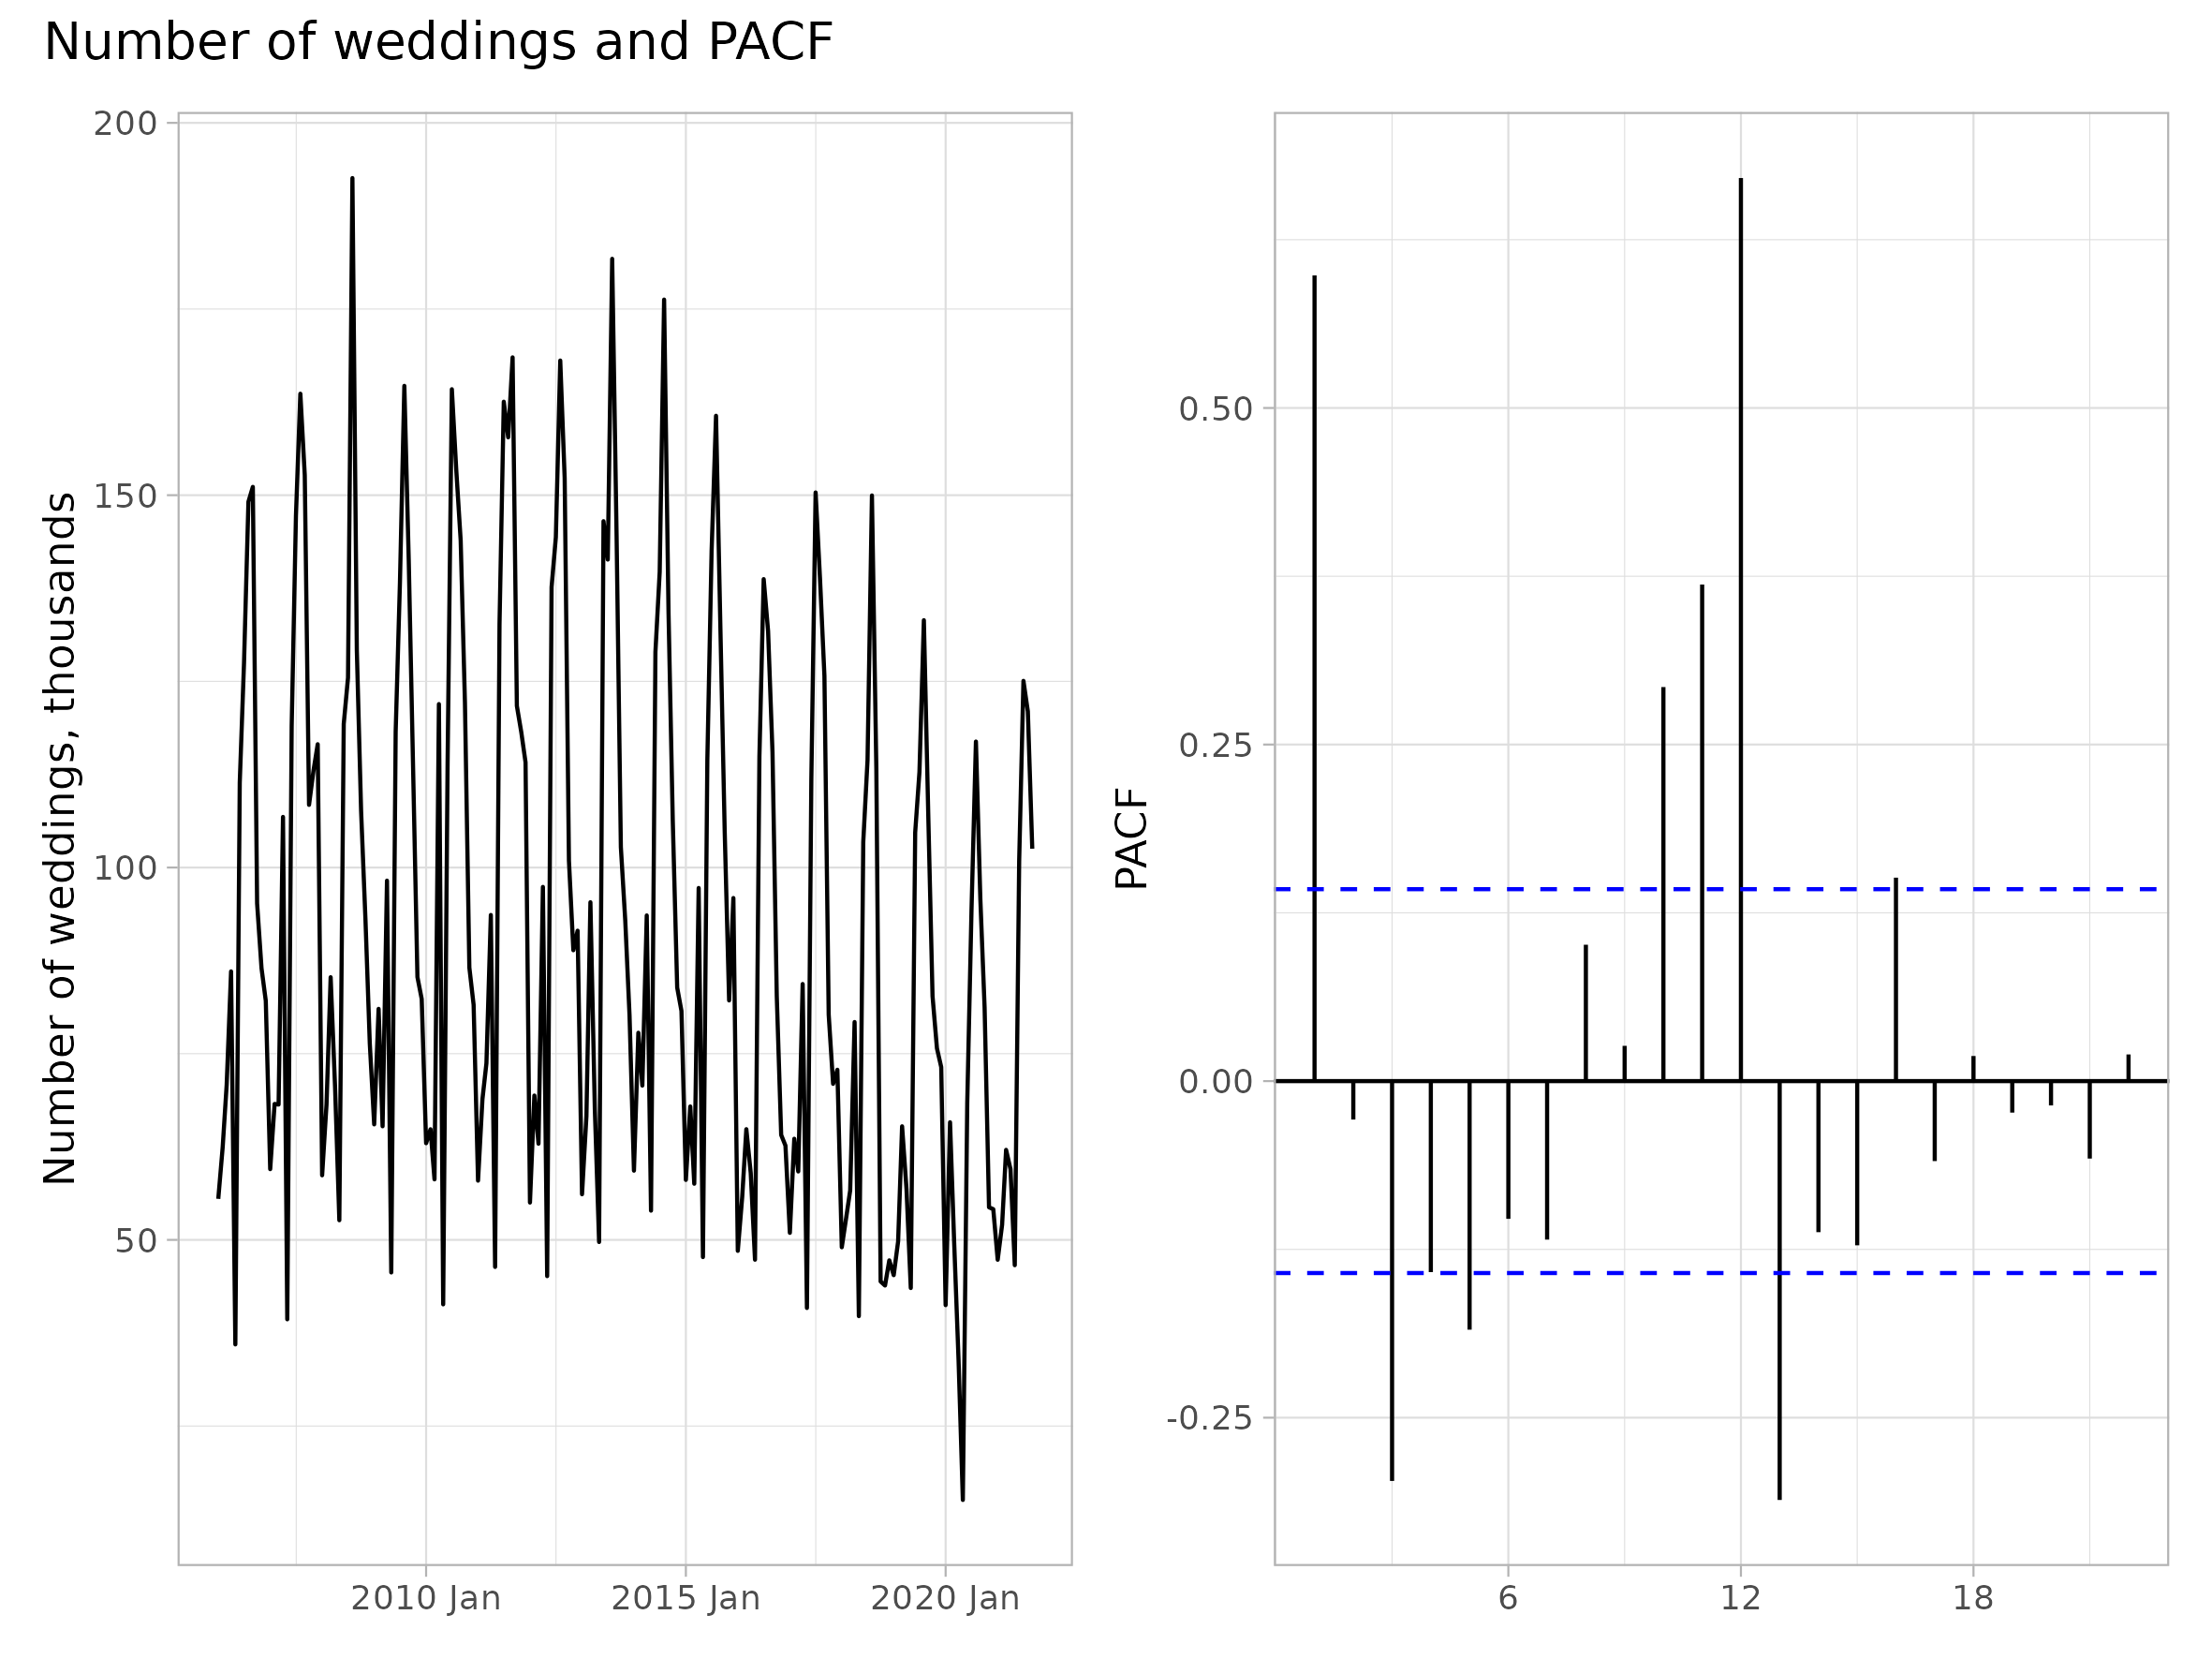
\includegraphics[width=\textwidth]{pictures/om_ts_01-127.png}
	
\end{frame}

\begin{frame}{Why is PACF a correlation?}
	
	\alert{Classic definition}
	
	\begin{block}{Custom PACF}
		$PACF_4$ — sample correlation between $a_t$ residuals and $b_t$ residuals:
		
		$a_t$ — regression residuals
		\[
		y_t \mid 1, y_{t-1}, y_{t-2}, y_{t-3};
		\]
		
		$b_t$ — regression residuals
		\[
		y_{t-4} \mid 1, y_{t-1}, y_{t-2}, y_{t-3}
		\]
	\end{block}
	
	\pause
	The difference between the definitions of \alert{small}
	
\end{frame}


\begin{frame}{STL features}
	
	\alert{Output:}
	\[
	y_t = T_t + S_t + R_t
	\]
	
	\pause
	Let's measure:
	\begin{itemize}
		\item Strength of $F_{trend}$ trend
		\item Strength of $F_{seas}$ seasonality
	\end{itemize}
	
\end{frame}

\begin{frame}{Strength of trend and seasonality}
	
	We got the decomposition:
	\[
	y_t = trend_t + seas_t + remainder_t.
	\]
	
	\pause
	\alert{Definition idea:}
	
	For an ideal decomposition with uncorrelated components:
	\[
	F_{trend} = \frac{\sVar(trend)}{\sVar(trend) + \sVar(remainder)},
	\]
	
	\pause
	\[
	F_{seas} = \frac{\sVar(seas)}{\sVar(seas) + \sVar(remainder)},
	\]
\end{frame}

\begin{frame}{Strength of trend and seasonality}
	
	We have the decomposition:
	\[
	y_t = trend_t + seas_t + remainder_t.
	\]
	
	\pause
	\alert{In practice}:
	\begin{itemize}[<+->]
		\item Trend strength:
		\[
		F_{trend} = \max\left\{1 - \frac{\sVar(remainder)}{\sVar(trend + remainder)}, 0 \right\}.
		\]
		\item Seasonality strength:
		\[
		F_{seas} = \max\left\{1 - \frac{\sVar(remainder)}{\sVar(seas + remainder)}, 0 \right\}.
		\]
		
	\end{itemize}
	
	
	
\end{frame}


\begin{frame}{Strength of trend and seasonality}
	
	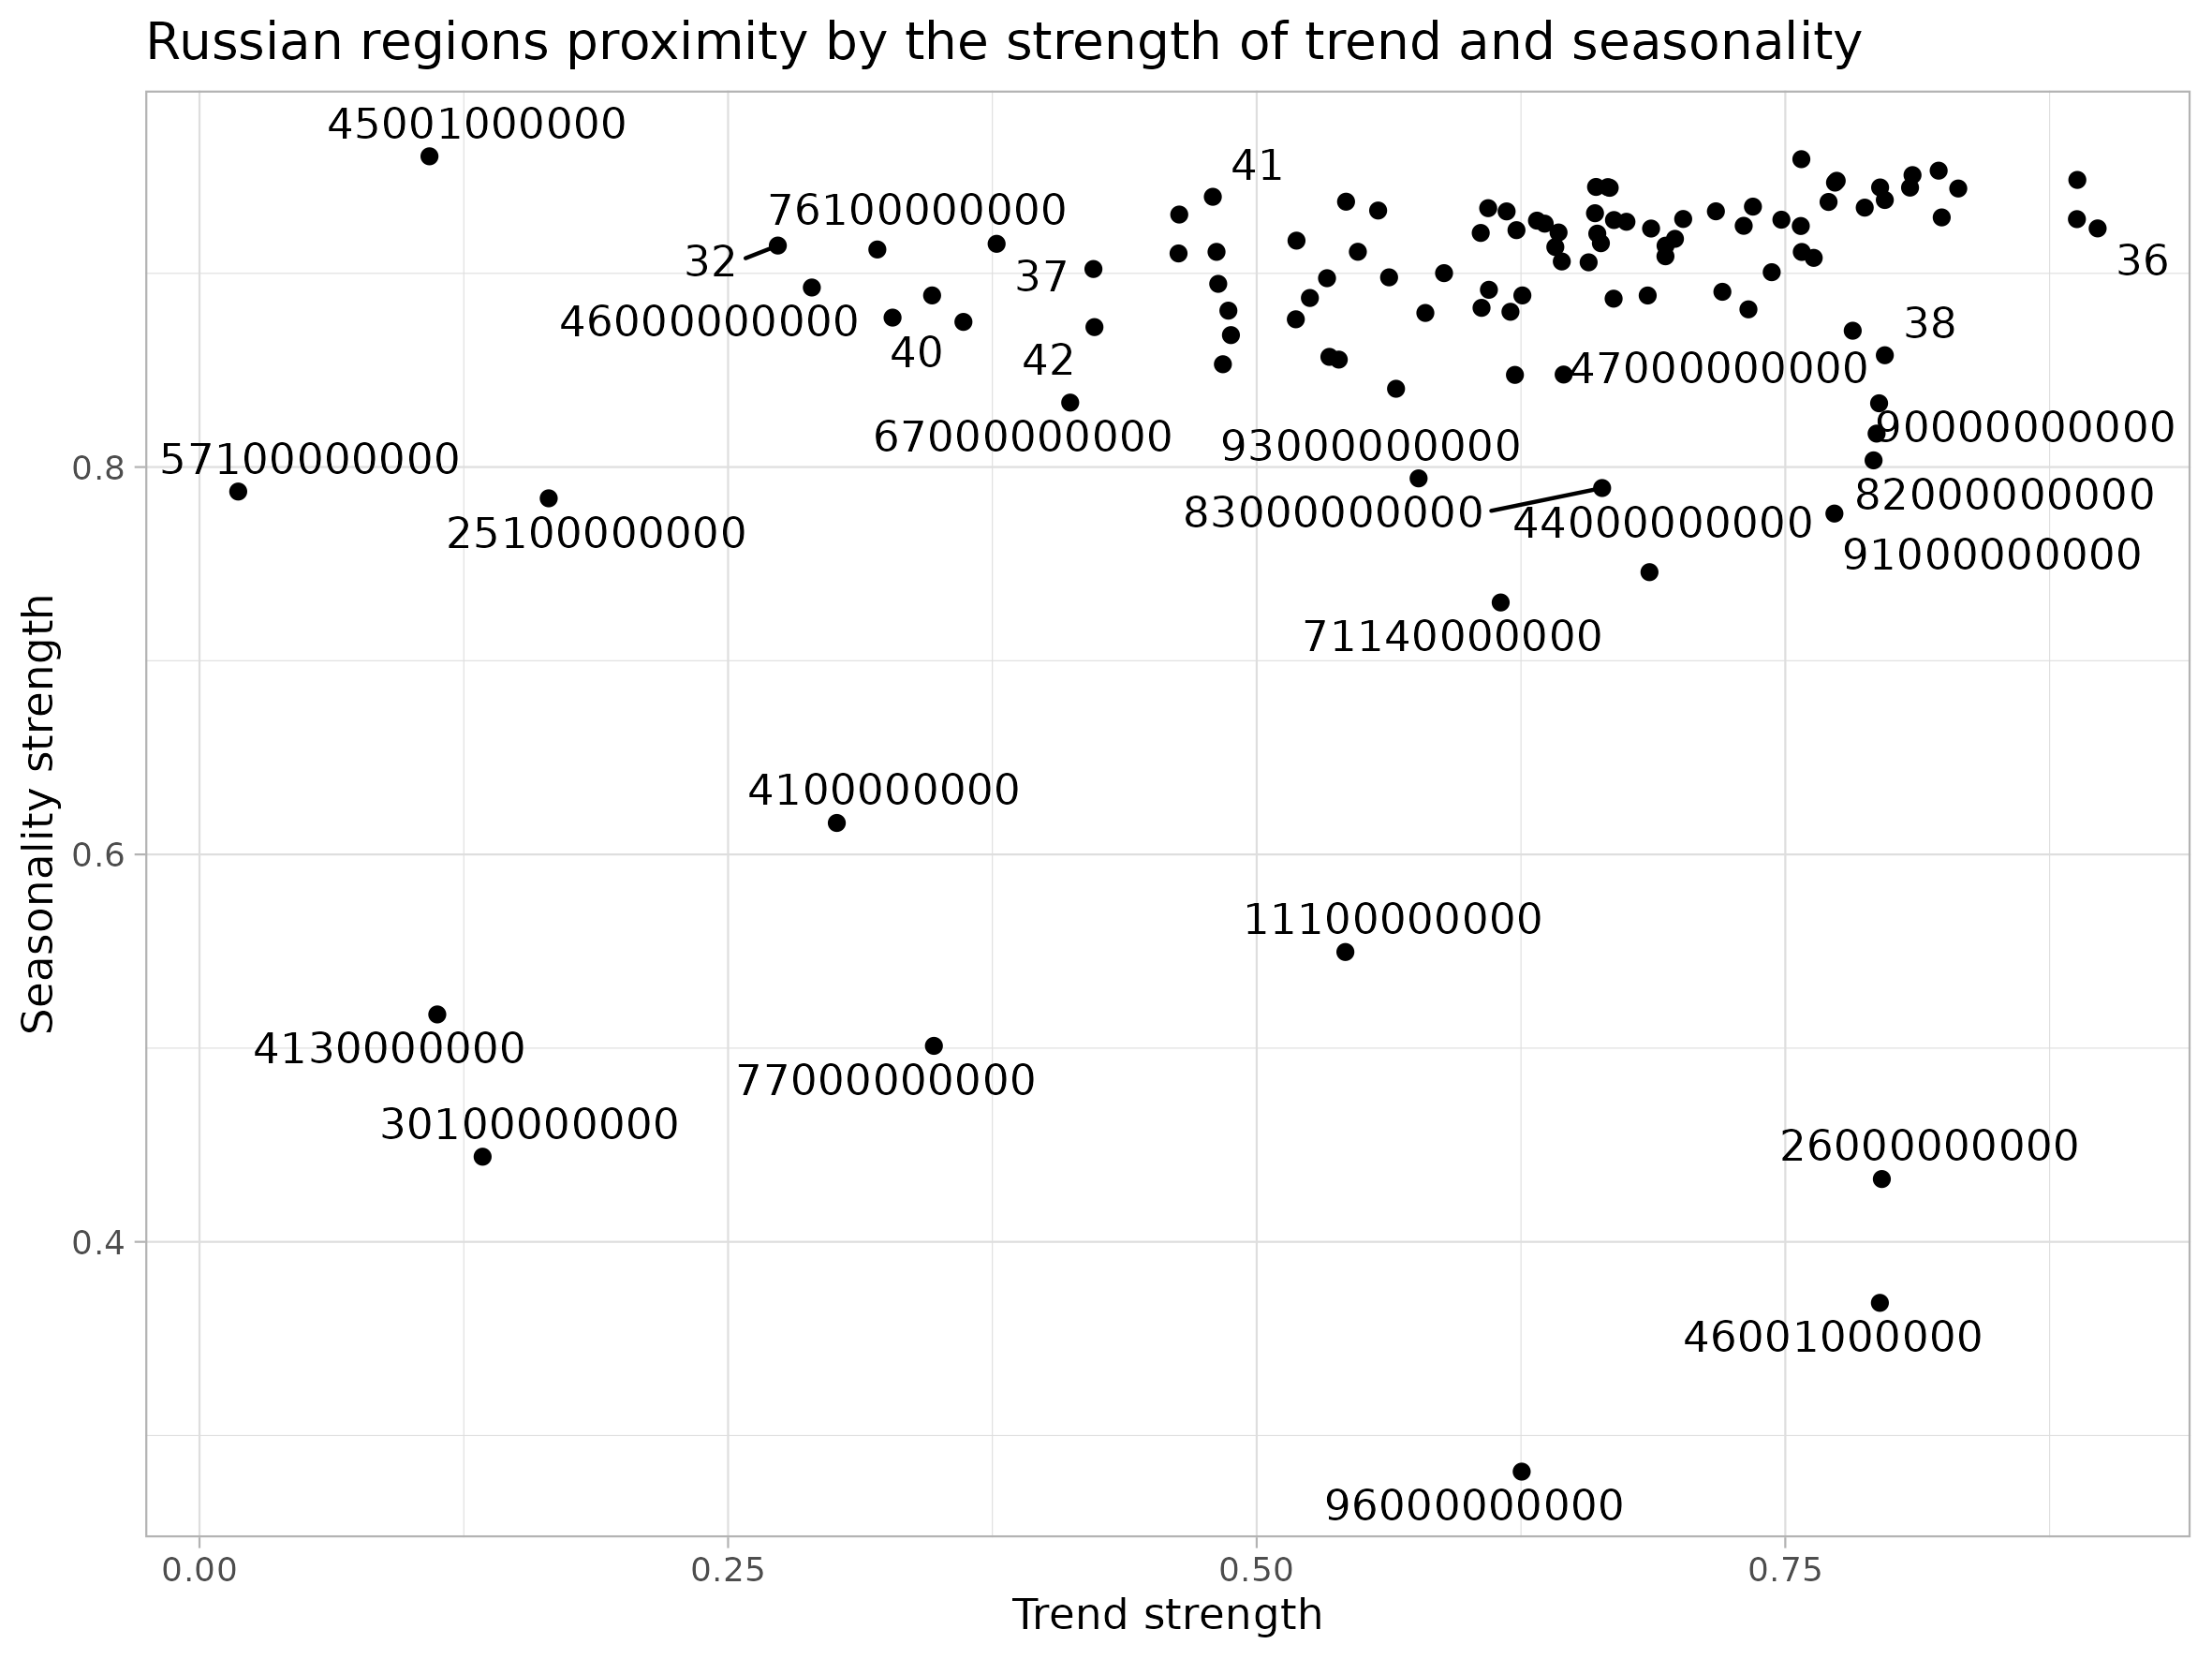
\includegraphics[width=\textwidth]{pictures/om_ts_01-138.png}
	
	
\end{frame}



\begin{frame}{Series Characteristics: Summary}
	
	\begin{itemize}[<+->]
		\item ACF — coefficients in \alert{paired} regressions or correlations
		\item PACF — coefficients in \alert{multiple} regressions or correlations
		\item STL allows you to measure \alert{strength of trend and seasonality} in comparison to the residual component
	\end{itemize}
\end{frame}
